\documentclass[a4paper, 12pt]{article}

\usepackage{lmodern}
\usepackage[french]{babel}
\usepackage[utf8]{inputenc}  
\usepackage[T1]{fontenc} 
\usepackage{float}
\usepackage{courier}
\usepackage{listings}
\usepackage{xcolor}
\usepackage{amsmath}
\usepackage{graphicx}
\usepackage{amsmath}       
\usepackage{hyperref}        
\usepackage{geometry}        
\geometry{top=2 cm, bottom=1.5 cm, left=1 cm, right=1 cm}

\begin{document}
 
\title{\textbf{Compte rendu UE Informatique}}
\author{COUËRON Lola \\ JOLY Marine \\ \\ L3 Physique, Université Grenoble Alpes}
\date{Novembre 2024}

\maketitle 


{
\hypersetup{hidelinks}

\renewcommand{\contentsname}{Sommaire}
\tableofcontents
}
%
%
%
%%% Chapitre1 %%%----------------------------------
\newpage
\section{Introduction}

\subsection{Contexte}	
	La simulation informatique est un outil prépondérant dans l’étude de phénomènes physiques. Elle permet de comparer des modèles théoriques et expérimentaux avec précision. Dans le cadre de l’UE Informatique nous présentons une simulation à N corps ainsi que deux exemples d'applications : un problème à deux corps et un système solaire.
L'objectif initial est de simuler l’interaction Terre - Soleil. Pour se faire nous utilisons le Principe Fondamental de la Dynamique de Newton qui nous permet d’obtenir les équations du mouvement. Cependant afin de décrire des systèmes plus complexes nous utilisons l’algorithme de Runge-Kutta d’ordre 4 qui permet de simuler l'interaction à N corps. Ces deux interactions sont visuellement décrite via l'outil PyGame.

\subsection{Structure générale du code}
	Ce projet étant collaboratif, nous avons travaillé sur\\ \href{https://github.com/MJ240103/solarSystem}{GitHub} (https://github.com/MJ240103/solarSystem) afin d'optimiser la répartition des tâches. Ce projet est divisé en 4 fichiers : \\
    \begin{enumerate}
        \item le fichier contenant l'application réalisée avec Tkinter (\textbf{UIsolarSystem.py})
        \item le fichier contenant la simulation réalisée avec PyGame (\textbf{mainEngine.py})
        \item le fichier contenant les équations et les paramètres physiques nécessaires à la simulation (\textbf{bodies.py})
        \item les fichier permettant de stocker les paramètres de simulations déjà existantes (fichiers json d'extension \textbf{.mj} et \textbf{Simulation1.py})
    \end{enumerate}
    \begin{figure}[H]
        \centering
        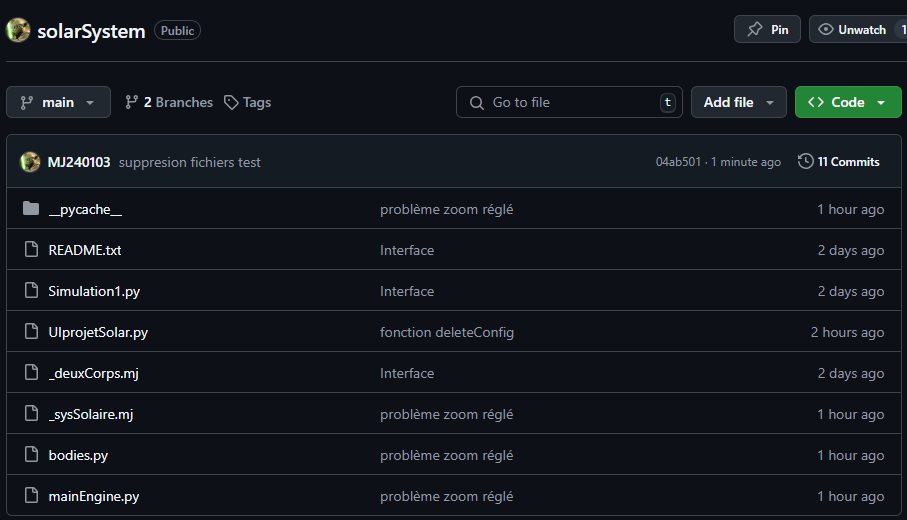
\includegraphics[width=0.45\linewidth]{img/imgGitHub.png}
        \caption{\label{fig:Git}Fichiers de la branche main du repository solarSystem.}
    \end{figure} 
     
	Le fichier \textbf{mainEngine.py} utilise les équations et paramètres physiques du fichier \textbf{bodies.py} afin de simuler les interactions attractives entre plusieurs corps et plusieurs paramètres par le biais de PyGame. Le nombre de corps et Les paramètres sont définis par l'utilisateur grâce à l'interface contenue dans le fichier \textbf{IUsolarSystem}. Celle-ci utilise Tkinter pour lancer la simulation PyGame. Les simulations peuvent être stockées dans des fichiers python (ex : \textbf{Simulation1.py}) ou dans des fichiers json (ex : \textbf{sysSolaire.mj)}.
%
%
%
%%% Chapitre2 %%% ----------------------------------
\newpage
\section{Physique}
%
%
\subsection{Implémentation naïve}	
	En premier lieu, nous utilisons une implémentation naïve des équations du mouvement. Nous considérons un corps central autour duquel gravite un autre corps. Le mouvement de ce corps est régi par la force de gravitation $\vec{F} = -G\frac{m_A m_B}{r^2} \vec{U_r}$. Les coordonnées cartésiennes sont utilisées afin de simplifier l'implémentation des équations du mouvement en Python. \\

La position d'une particule en coordonnées cartésiennes est donnée par :
        \begin{equation}
            \vec{r}(t) = x(t) \vec{i} + y(t) \vec{j} + z(t) \vec{k} 
        \end{equation} 
La vitesse est la dérivée de la position par rapport au temps :
        \begin{equation}
            \vec{v}(t) = \frac{d\vec{r}(t)}{dt} = \frac{dx(t)}{dt} \vec{i} + \frac{dy(t)}{dt} \vec{j} + \frac{dz(t)}{dt} \vec{k}
        \end{equation} \\    
L'accélération est la dérivée de la vitesse par rapport au temps :
        \begin{equation}
            \vec{a}(t) = \frac{d\vec{v}(t)}{dt} = \frac{d^2x(t)}{dt^2} \vec{i} + \frac{d^2y(t)}{dt^2} \vec{j} + \frac{d^2z(t)}{dt^2} \vec{k}
        \end{equation}

Pour obtenir les équations du mouvement, on applique le Principe Fondamental de la Dynamique (PFD) de Newton et on projette les forces en cartésien : $\vec{F} = m \vec{a}$ \\

        
Enfin, nous implantons ces équations en Python. L'appel à la fonction \texttt{applyGravity} effectue les calculs de position, de vitesse et d'accélération du corps en orbite. Quant à la fonction \texttt{setPosition}, celle-ci est chargée de mettre à jour la position du corps en orbite en fonction de sa vitesse et de l'intervalle de temps indiquant la durée d'une révolution autour de l'astre central. 

    \begin{figure}[H]
		\centering
		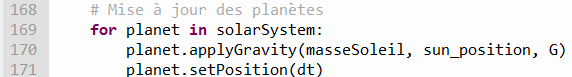
\includegraphics[width=0.4\linewidth]{img/naifMain.png}
		\caption{\label{fig: naifMain }Execution de \texttt{applyGravity} et \texttt{setPosition} afin de générer les coordonnées des corps}  
	\end{figure}
	\begin{figure}[H]
		\centering
		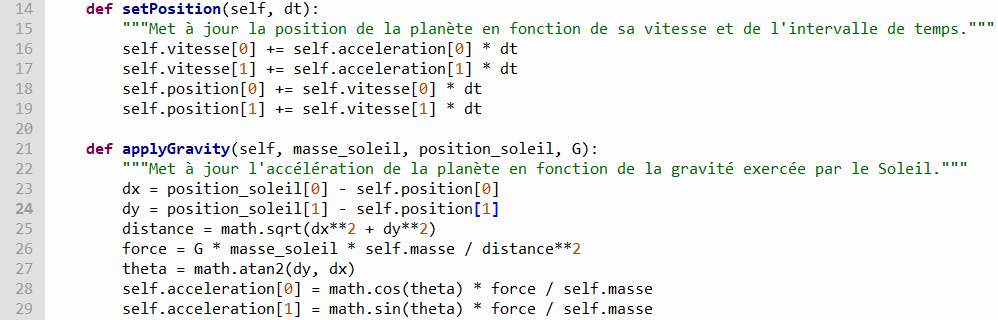
\includegraphics[width=0.4\linewidth]{img/naif.png}
		\caption{\label{fig: ETape2 Rk4}Fonctions \texttt{setPosition} et \texttt{applyGravity} du module bodies.py}
	\end{figure}
	
	Ces fonctions ne sont pas présente dans le code final car elles sont désormais remplacées par de nouvelles fonctions utiles pour une implémentation Runge-Kutta d'ordre 4.\

\texttt{applyGravity} est désormais rémplacée par \texttt{gravite} et \texttt{setPosition} par \texttt{selfDraw} .
%
%
\newpage   
\subsection{Implémentation Runge-Kutta ordre 4}

	L'implémentation naïve étant un outil limité nous utilisons l'algorithme de Runge-Kutta d'ordre 4 (RK4) afin de décrire des systèmes plus complexes comme l'interaction entre plusieurs corps. La méthode d’Euler ou bien celle de Runge-Kutta d’ordre 4 semble ainsi plus adaptées. \\

	La méthode d'Euler permet à partir d'une condition initiale de résoudre une équation différentielle du premier ordre. Cette méthode est simple mais peu précise notamment lorsque l'on choisit des pas trop grand car son erreur est de l'ordre de $h$ (avec h le pas). C'est pourquoi si l'on divise le pas par 2 l'erreur est divisée par 2. \\

Par conséquent, du fait de sa précision la méthode RK4 a retenu toute notre attention. En effet, cette méthode utilise des itérations. La première solution éstimée est utilisée pour éstimer une deuxième solution plus précise, et ainsi de suite. La méthode RK4 est une méthode d'ordre 4, ce qui signifie que l'erreur totale accumulée est de l'ordre de $h^4$. Donc si on divise le pas par 2, l’erreur est divisée par 16. Ainsi, RK4 est plus précise que la méthode d'Euler. \\

	On considère le problème suivant : $y' = f(t,y)$ avec $y(t_0) = y_0$. \\
	
La méthode RK4 est donnée par l'équation : $y_{n+1} = y_n + \frac{h}{6} (k_1 + 2k_2 + 2k_3 + k_4)$ où \\
            
	\begin{itemize}
		\item $k_1 = f(t_n, y_n)$ \\
		\item $k_2 = f(t_n + \frac{h}{2}, y_n + \frac{h}{2} k_1)$ \\
		\item $k_3 = f(t_n + \frac{h}{2}, y_n + \frac{h}{2} k_2)$ \\
		\item $k_4 = f(t_n + h, y_n + hk_3)$ \\
	\end{itemize} 
	
	Le fonctionnement se base sur l'idée que la valeur suivante ($y_{n+1}$) est approchée par la somme de la valeur courante ($y_n$) et du produit de la taille de l'intervalle (h) par la pente estimée. Cette pente est obtenue en effectuant une moyenne pondérée des pentes : \\

	\begin{itemize}
		\item $k_1$ correspond à la pente au début de l'intervalle. 
	\begin{figure}[H]
		\centering
		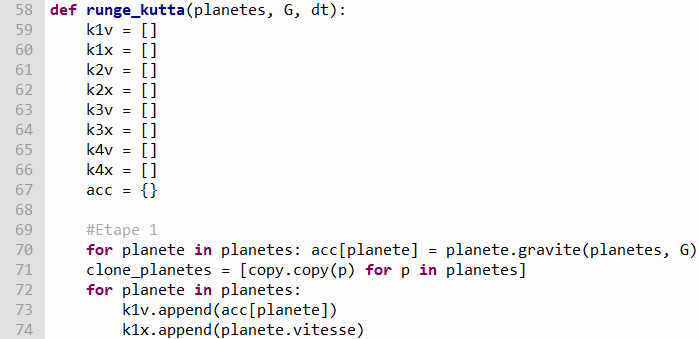
\includegraphics[width=0.4\linewidth]{img/RK4partie1.png}
		\caption{\label{fig: ETape1 Rk4}Etape 1 de la méthode RK4.}  
	\end{figure}	
	
\item  $k_2$ correspond à la pente au milieu de l'intervalle. Elle s'obtient en utilisant $k_1$ pour calculer la valeur de $y$ au point $t_n + \frac{h}{2}$ par le biais de la méthode d'Euler.
	\begin{figure}[H]
		\centering
		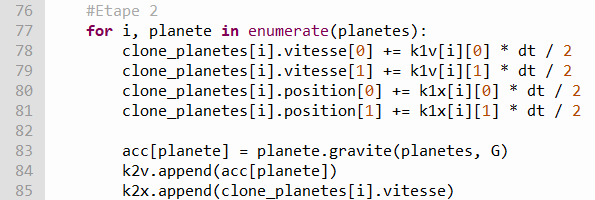
\includegraphics[width=0.4\linewidth]{img/RK4partie2.png}
		\caption{\label{fig: ETape2 Rk4}Etape 2 de la méthode RK4.}  
	\end{figure}
	
\item $k_3$ est la pente au milieu de l'intervalle, mais obtenue en utilisant $k_2$ pour $y$.
	\begin{figure}[H]
		\centering
		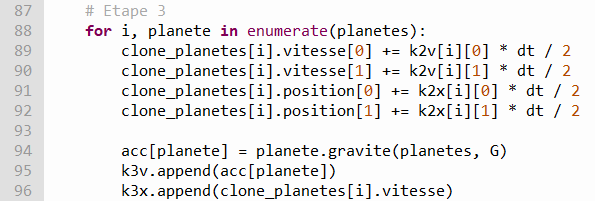
\includegraphics[width=0.4\linewidth]{img/RK4partie3.png}
		\caption{\label{fig: ETape3 Rk4}Etape 3 de la méthode RK4.}  
	\end{figure}
	
\item $k_4$ correspond à la pente de la fin de l'intervalle, obtenue avec la valeur de $y$ calculée en utlisant $k_3$.
	\begin{figure}[H]
		\centering
		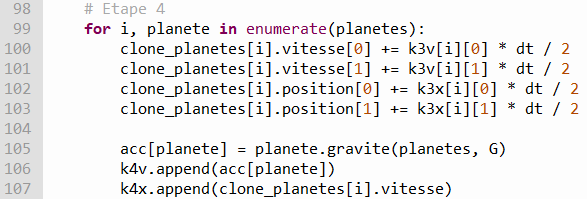
\includegraphics[width=0.4\linewidth]{img/RK4partie4.png}
		\caption{\label{fig: ETape4 Rk4}Etape 4 de la méthode RK4.}  
	\end{figure}
	 
Lorsque la moyenne pondérée des 4 pentes est effectuée, un poids plus important est donné aux pentes du milieu.
	\begin{figure}[H]
		\centering
		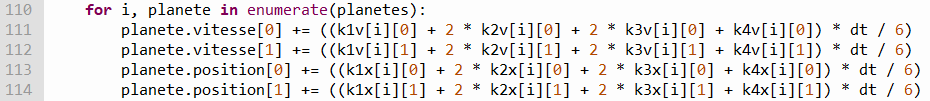
\includegraphics[width=0.4\linewidth]{img/RK4partiefin.png}
		\caption{\label{fig: ETapeFin Rk4} Itération de la méthode RK4.}  
	\end{figure}
    \end{itemize} 
  
%
%
%              
%%% Chapitre3 %%% ----------------------------------
\section{Interface graphique de l'application de simulation}
%
%

\subsection{Paramétrage des simulations}

\subsubsection{Body}
Nous appelons \texttt{Body} un objet regroupant les caractéristiques suivante: 

    \begin{itemize}
        \item Nom (string) : Nom de l'objet
        \item Masse (float) : Masse de l'objet
        \item Rayon (float) : Rayon de l'objet
        \item Position (float tuple) : Position (cartésienne) de l'objet
        \item Vitesse (float tuple) : Vitesse (cartésienne) de l'objet
        \item Acceleration (float tuple) : Accélération (cartésienne) de l'objet
        \item couleur ( int 3-uplet) : Couleur \\
    \end{itemize} 

Un \texttt{Body} peut par exemple représenter la Terre, le Soleil ou bien un satellite artificiel. 

\subsubsection{Simulation}
Nous appelons \texttt{Simulation} un objet regroupant les caractéristiques suivantes: 

    \begin{itemize}
        \item Nom\_Simu (string) : Nom de la simulation
        \item FPS (int) : Frame Per Second (nombre d'image par seconde) de la simulation
        \item G (float) : Constante gravitationnelle
        \item dt (float) : Intervalle de temps utilisé par RK4
        \item SPACE\_X (float) : Taille horizontale de l'espace simulé
        \item SPACE\_Y (float) : Taille vecticale de l'espace simulé
        \item ECHELLE\_RAYON (float) : Echelle de rendu des rayons des \texttt{body}
        \item UNIVERSE\_CENTER (float tuple) : Centre de l'univers (au centre de l'affichage en début de simulation)
        \item planetes (\texttt{Bodylst}) : Liste des objets, tels que définit avec le constructeur \texttt{body}\\ 
    \end{itemize} 

Pour enregistrer une simulation, nous utilisons le format \texttt{JavaScript Object Notation} (JSON).\\ 

Python a l'avantage de directement prendre en charge ce format à l'aide du module Json. Ainsi, en important le fichier simulation et en signifiant à python qu'il s'agit de json, on peut accéder aux différents paramètres de la simulation. \\

On accède par exemple au nom d'une simulation représentée par la variable sim de la manière suivante: nomSimu = sim["Nom\_Simu"] (voir Figure 9). \\

Nous transformons ensuite notre objet directement convertis depuis le Json en un objet Simulation à l'aide d'une classe. L'avantage de cette méthode est que la classe Simulation possède une méthode \texttt{launch()} qui lance directement l'exécution de la simulation dans le moteur. (voir Figure 10)

	
	\begin{figure}[H]
    	\centering
    	\begin{minipage}{0.5\linewidth}
        	\centering
        	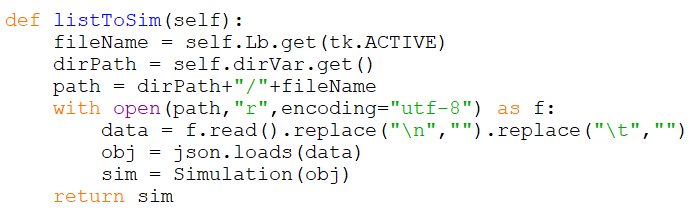
\includegraphics[width=\linewidth]{img/toJson.png}
        	\caption{\label{fig:TOJSON} Importation d'un fichier via le module Json}
    	\end{minipage}
    	\hspace{0.05\linewidth}  % Espace horizontal entre les deux images
    	\begin{minipage}{0.38\linewidth}
        	\centering
        	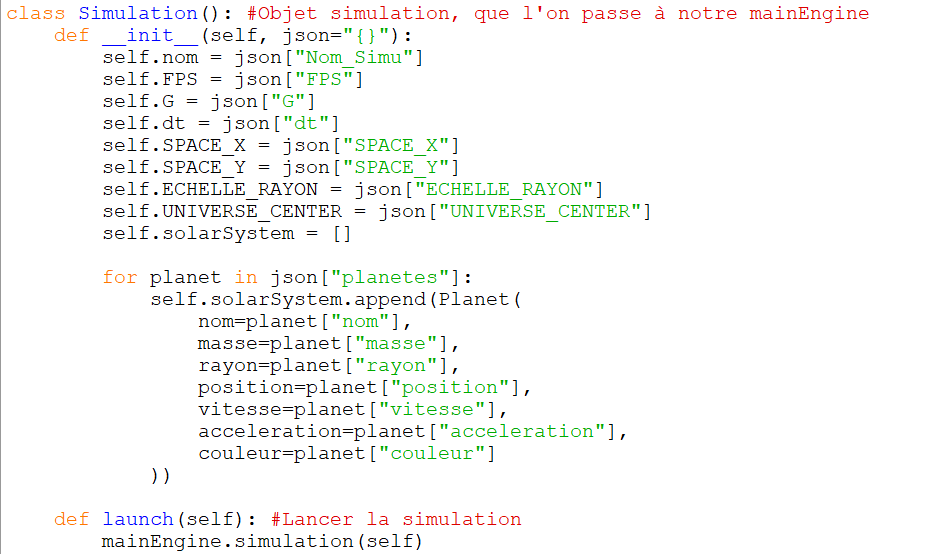
\includegraphics[width=\linewidth]{img/simulationClasse.png}
        	\caption{\label{fig:simClasse} Classe simulation} 
    	\end{minipage}
	\end{figure}
%
%
\subsection{Modification, Création}
	L'interface, réalisée à l'aide de Tkinter se présente comme suit:
    \begin{figure}[H]
		\centering
		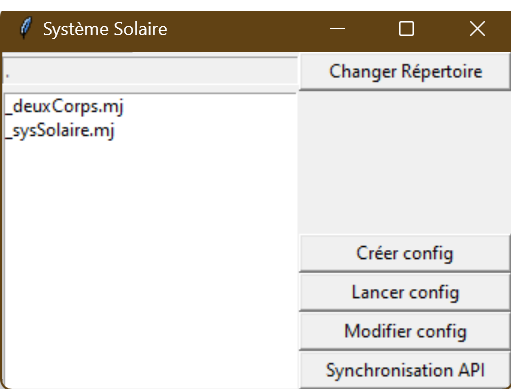
\includegraphics[width=0.2\linewidth]{img/mainInterface.png}
		\caption{\label{fig: IntMain} Interface Fenêtre - principale}  
	\end{figure}

    Sur la fenêtre principale de l'interface, on a la possibilité de se placer dans un répertoire en cliquant sur "Changer Répertoire". Le répertoire par défaut est celui du fichier interface. 

    La \texttt{ListBox} à gauche liste les fichiers de simulations compatibles (.mj) dans le répertoire courant. Ces fichiers contiennent un code JSON correspondants à l'objet \texttt{Simulation} définit plus haut. \\

    Lorsqu'on clique sur le nom d'un fichier, il devient le fichier actif. On peut ensuite cliquer sur:

    \begin{itemize}
        \item "Lancer config" : Exécute la configuration dans l'engine
        \item "Modifier config" : Ouvre la fenêtre secondaire avec les paramètres de la simulation active. \\
    \end{itemize}

    Indépendamment du fichier actif, on peut cliquer sur:

    \begin{itemize}
        \item "Créér config" : Ouvre la fenêtre secondaire avec les paramètres par défaut.
        \item "Synchronisation API" : Récupère les positions et vitesse actuelles des astres du système solaire , créé un fichier de simulation, et l'execute.
    \end{itemize}

    \begin{figure}[H]
		\centering
		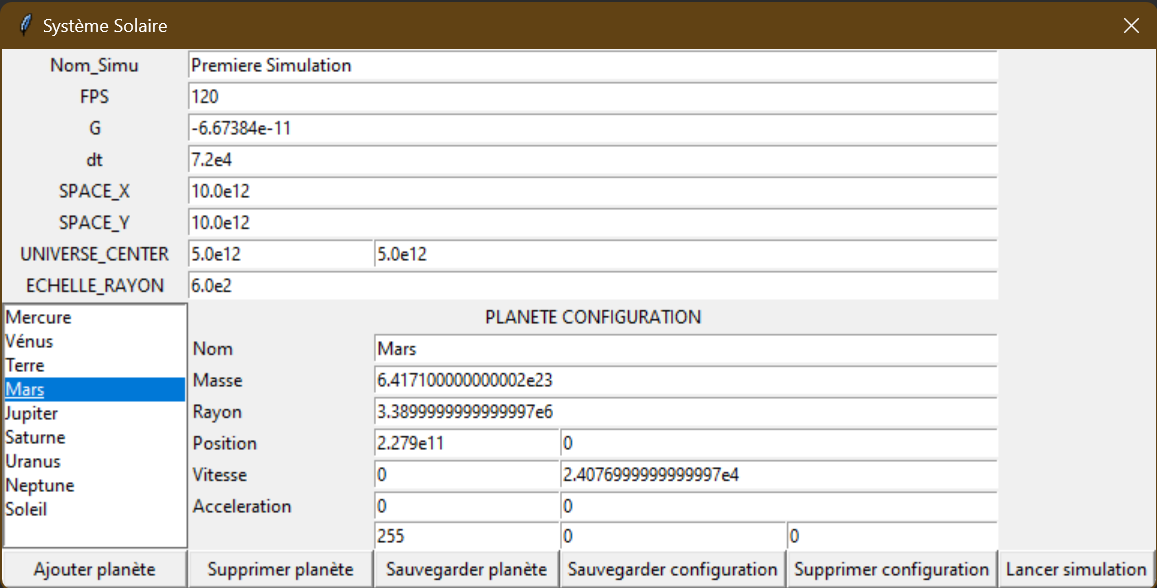
\includegraphics[width=0.4\linewidth]{img/interfaceFenetreSecondaire.png}
		\caption{\label{fig: IntSec} Interface Fenêtre - secondaire}  
	\end{figure}

    Une fenêtre secondaire s'ouvre lors de la création ou de la modification d'une simulation, avec le même comportement dans les deux cas. Les constantes peuvent être modifiées en ajustant directement les champs correspondants. 
    
	Pour éditer une planète, il suffit de cliquer sur son nom, de modifier les champs, puis de valider en cliquant sur "Sauvegarder planète". Il est aussi possible d'ajouter ou de supprimer une planète.\\
	
	Une fois les modifications terminées, on clique sur "Sauvegarder configuration", qui permet de sauvegarder la simulation via une fenêtre de dialogue. Il est possible d'écraser l'ancienne version ou de lancer la simulation. Avant la sauvegarde, on peut tester la simulation en cliquant sur "Lancer Simulation"
.


%%% Chapitre4 %%% ----------------------------------
\section{Interface graphique de la simulation par le biais d'exemples d'utilisation} 
Comme explicité en 2.2, on utilise RK4 dont la mise à jour en temps réelle permet la détermination des trajectoires.

\subsection{Simulation à deux corps}
\subsubsection{Mise à jour de Runge-Kutta}
La simulation des mouvements des corps est effectuée à chaque itération de la boucle principale. La méthode de Runge-Kutta est utilisée pour mettre à jour les positions des planètes en fonction des forces gravitationnelles. Cela se produit à la ligne 120 : \texttt{runge\_kutta(config.solarSystem, config.G, config.dt)}

\subsubsection{Affichage}
La fonction \texttt{realToDisplay} transforme les coordonnées réelles (en fonction de l'espace simulé) en coordonnées adaptées à l'affichage sur la fenêtre Pygame. Ensuite, la méthode \texttt{selfDraw} de l'instance de la classe \texttt{Planet} est utilisée pour afficher la simulation à l'écran.

	\begin{figure}[H]
    	\centering
        \begin{minipage}{0.2\linewidth}
        	\centering
        	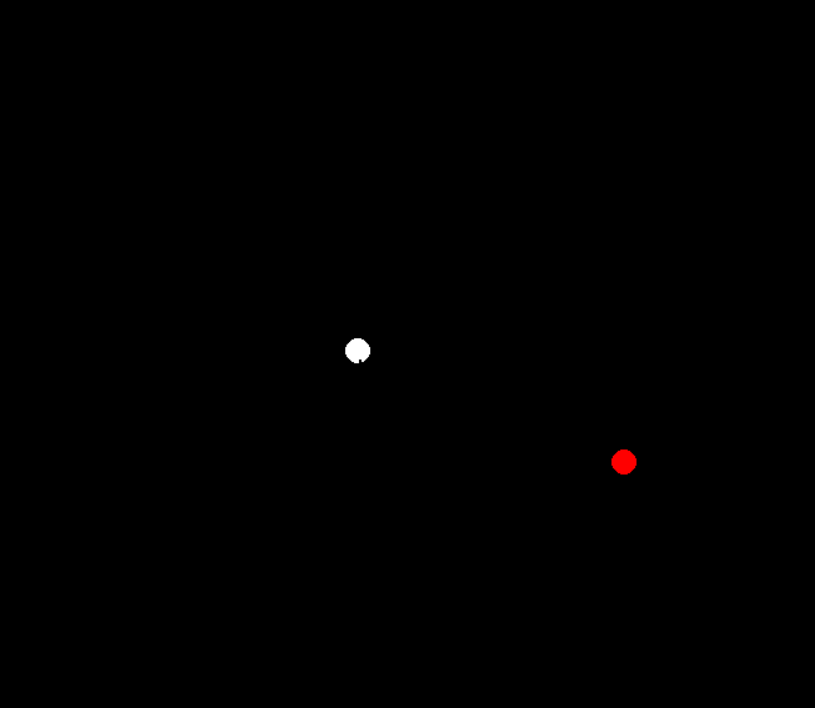
\includegraphics[width=\linewidth]{img/couverture.png}
        	\caption{\label{fig:DeuxCorps1} Interaction deux corps sans trace}
    	\end{minipage}
        \hspace{0.05\linewidth}  % Espace horizontal entre les deux images
    	\begin{minipage}{0.2\linewidth}
        	\centering
        	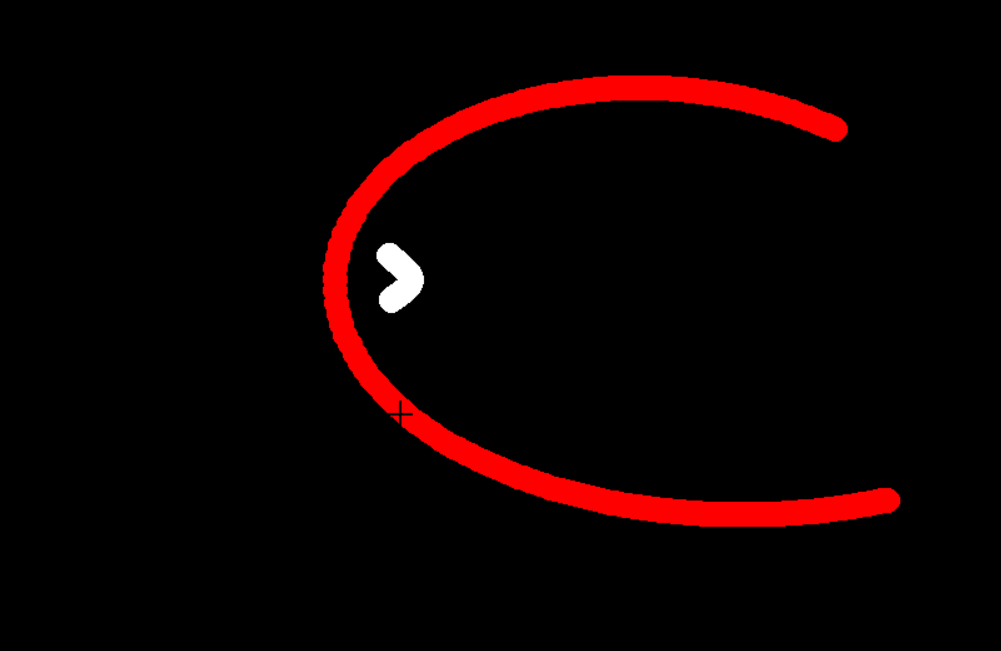
\includegraphics[width=\linewidth]{img/interactionDeuxCorps.png}
        	\caption{\label{fig:DeuxCorps2} Interaction deux corps avec trace}
    	\end{minipage}
    	\hspace{0.05\linewidth}  % Espace horizontal entre les deux images
    	\begin{minipage}{0.2\linewidth}
        	\centering
        	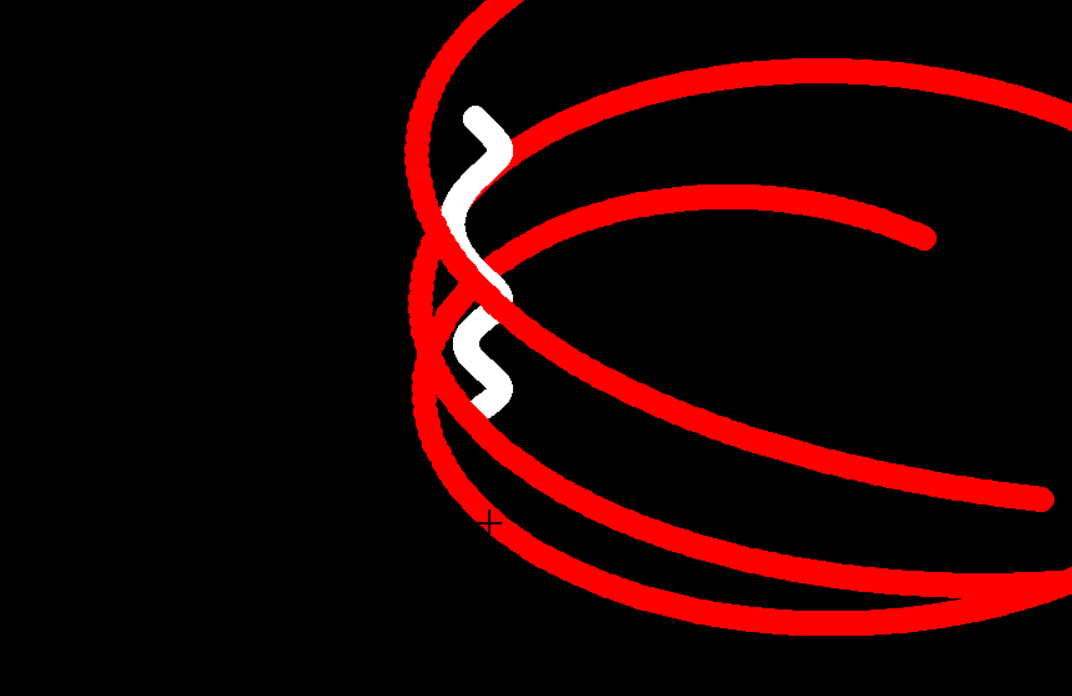
\includegraphics[width=\linewidth]{img/interactionDeuxCorps2.png}
        	\caption{\label{fig:DeuxCorps3} Evolution de l'interaction deux corps} 
    	\end{minipage}
	\end{figure} 

On peut aussi déplacer la caméra par rapport au centre de l'écran en utilisant les touches (z, q, s et d).
\paragraph{}
Au lancement de la simulation, les trajectoires des corps ne sont pas affichées. Toutefois, en appuyant sur la touche espace du clavier, il est possible de les afficher ou de les supprimer. En effet, appuyer sur espace permet de choisir si l'on veut remplir le fond en noir ou non à chaque mise à jour de la position des corps.

\begin{figure}[H]
		\centering
		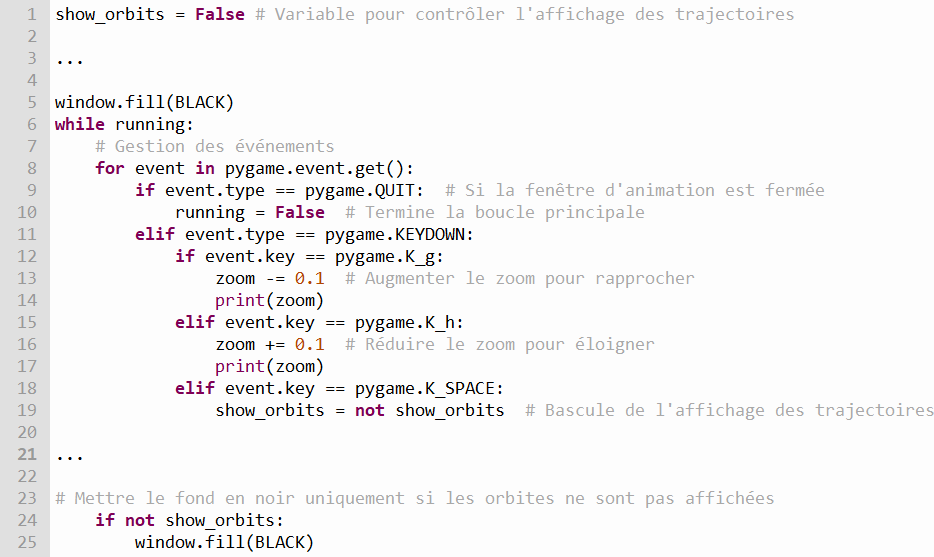
\includegraphics[width=0.4\linewidth]{img/codeTrajectoire.png}
		\caption{\label{fig: Source} Code source du tracé des trajectoires}  
	\end{figure}


\subsubsection{Option ZOOM}
On utilise les touches (g,h) pour zoomer/dézoomer. Cette fonctionnalité est rendue possible par les lignes suivantes :

	\begin{figure}[H]
		\centering
		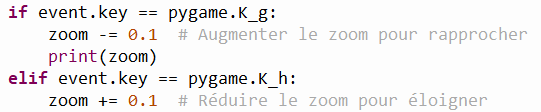
\includegraphics[width=0.4\linewidth]{img/optionZoom.png}
		\caption{\label{fig: Source} Code source de la fonctionnalité}  
	\end{figure}

Le zoom influence la manière dont les positions des planètes sont converties pour l'affichage à l'écran. Cette transformation est effectuée dans la méthode \texttt{planet.selfDraw()}, qui prend en compte la valeur du zoom pour ajuster la taille et la position des planètes dans la fenêtre Pygame.

	\begin{figure}[H]
		\centering
		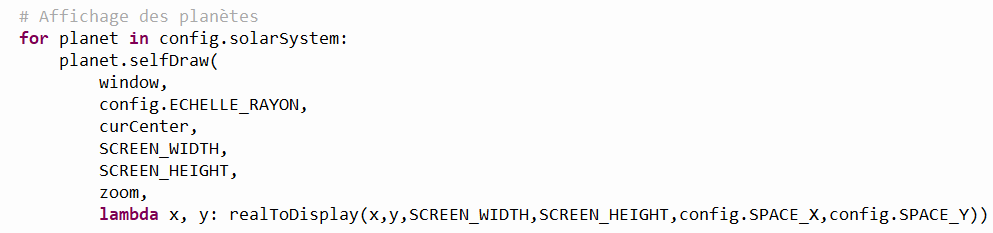
\includegraphics[width=0.5\linewidth]{img/priseEnCompte.png}
		\caption{\label{fig: priseEnCompte} Prise en compte de la fonctionnalité zoom}  
	\end{figure}
	
La fonction lambda \texttt{realToDisplay()} calcule les nouvelles positions des objets en fonction de l'échelle du zoom, permettant de zoomer à l'intérieur ou à l'extérieur du système solaire simulé tout en ajustant l'affichage de manière cohérente. 

\subsubsection{Choix d'une planète centrale}
On peut choisir laquelle des deux planètes est placée au centre du système.

	\begin{figure}[H]
    	\centering
    	\begin{minipage}{0.27\linewidth}
        	\centering
        	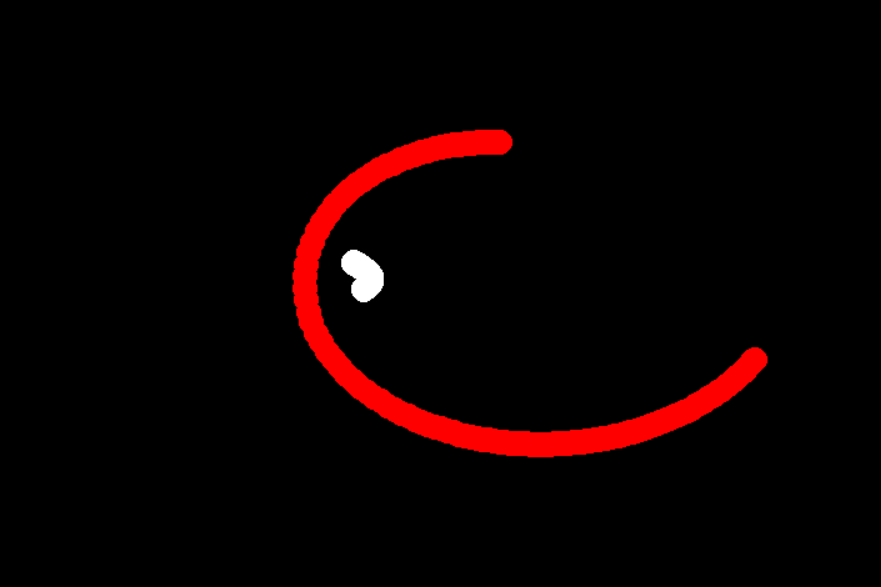
\includegraphics[width=\linewidth]{img/centrage1.png}
        	\caption{\label{fig:centrage1} Centrage 1}
    	\end{minipage}
    	\hspace{0.05\linewidth}  % Espace horizontal entre les deux images
    	\begin{minipage}{0.27\linewidth}
        	\centering
        	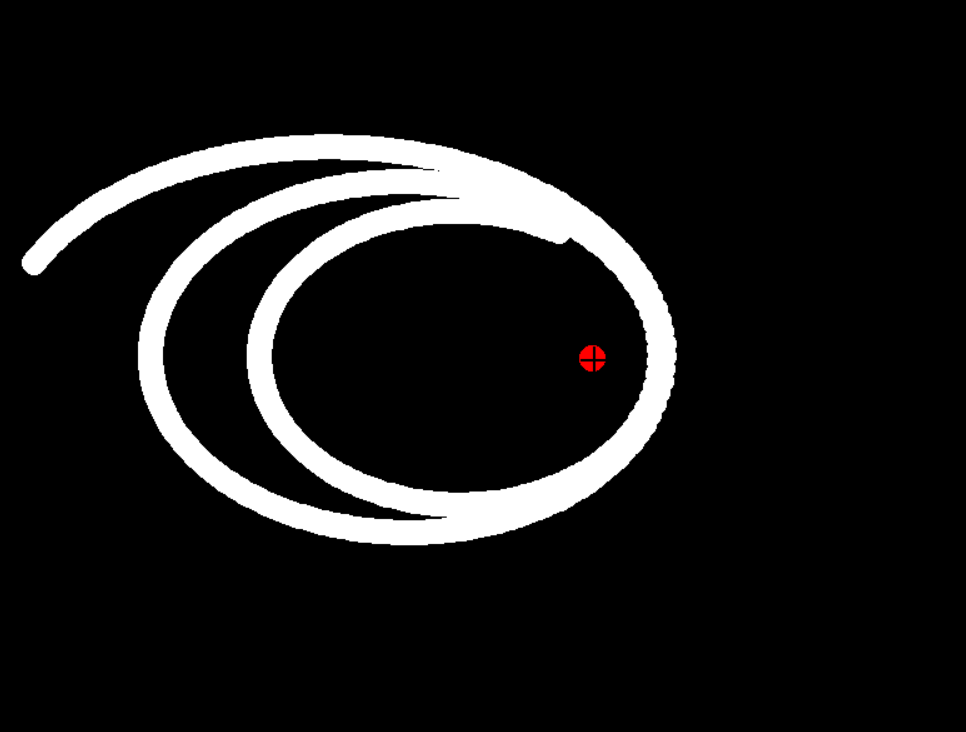
\includegraphics[width=\linewidth]{img/centrage2.png}
        	\caption{\label{fig:centrage2} Centrage 2} 
    	\end{minipage}
	\end{figure} 


\subsection{Simulation du système solaire}
Tout ce qui à été décrit précédemment est valable dans la simulation du système solaire.
A partir de l'interface principale de la fenêtre Tkinter on peut lancer la simulation \texttt{sysSolaire}.On utilise le fichier \texttt{sysSolaire.mj} de type JSON qui contient les caractéristiques d'une simulation du système solaire. On peut également la modifier pour y ajouter d'autres corps tels que les lunes de Jupiter.

	\begin{figure}[H]
		\centering
		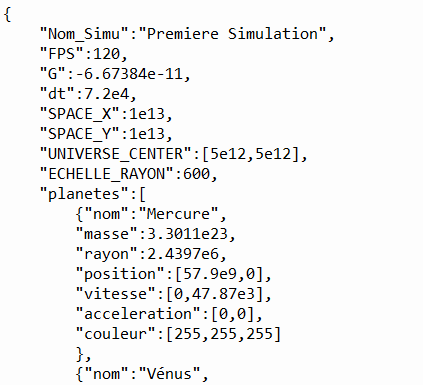
\includegraphics[width=0.27\linewidth]{img/json.png}
		\caption{\label{fig: json} Fichier JSON}  
	\end{figure}
	

La simulation du système solaire permet de mettre en évidence le caractère attracteur du Soleil du fait de sa masse prépondérante par rapport aux autres corps ainsi que les trajectoires cycloïdales des planètes lorsque l'on change de référentiel d'observation.
	\begin{figure}[H]
    	\centering
    	\begin{minipage}{0.3\linewidth}
        	\centering
        	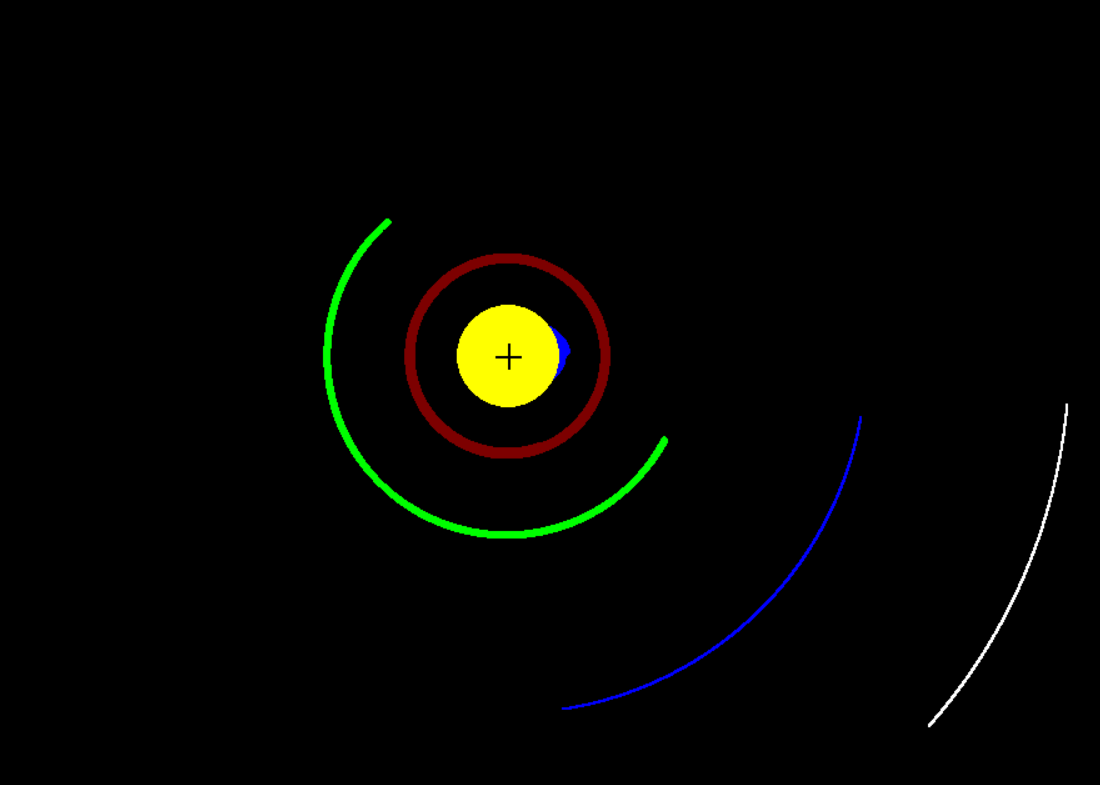
\includegraphics[width=\linewidth]{img/systemeSolaireCentrage1.png}
        	\caption{\label{fig:systsolaire1} Centrage Soleil}
    	\end{minipage}
    	\hspace{0.05\linewidth}  % Espace horizontal entre les deux images
    	\begin{minipage}{0.27\linewidth}
        	\centering
        	\includegraphics[width=\linewidth]{img/systemesolaireCentrage2.png}
        	\caption{\label{fig:systsolaire2} Changement de configuration} 
    	\end{minipage}
	\end{figure} 

%%% Chapitre5 %%% ----------------------------------
%\newgeometry{top=2 cm, bottom=2 cm, left=1.5 cm, right=1.5 cm}
\section{Conclusion}
\subsection{Extension du programme}
Il est possible de simuler n'importe quel système mécanique avec notre application puisque le RK4 est indépendant de la force utilisée. On pourrait par exemple simuler l'intéraction de 42 particules avec différentes charges.

\subsection{Conclusion}
Ce projet nous a permis de calculer et simuler des intéractions gravitationnelles entre différents corps. 
La méthode de résolution des équations différentielles RK4 s’est montrée efficace et suffisante afin d’obtenir un niveau de précision conséquent. 
Cet algorithme est indépendant du nombre d’objet contenu dans l’ensemble du système et des expressions des différentes forces qui s'appliquent au système. C’est pourquoi il est aisé de généraliser l’interaction de deux corps à N corps.\\

Enfin, l’outil d’interface graphique PyGame à permis de mettre en évidence certaines caractéristiques.
C’est notamment le cas de la vitesse de la trajectoire elliptique en fonction de la distance corps central - corps en orbite (système deux corps).
On a aussi pu observer l’influence de la masse d’un corps sur les autres et l'influence du centrage concernant le corps le plus massif (système N corps, Figure 21).\\

Par conséquent, cet outil est très utile dans un but pédagogique puisqu'il permet de mettre en mouvement des équations qui peuvent sembler abstraites aux premiers abords. \\

Toutefois, afin d'améliorer cette application, nous pourrions tenir compte de l'impact de la collision entre deux corps. De plus, dans le cas du système solaire, nous pourrions utiliser une API afin de récupérer des données précises concernant les positions et vitesses des corps.

\end{document}